\documentclass[crop=true]{standalone}
\usepackage[subpreambles=true]{standalone}
\usepackage{tikz}

\begin{document}
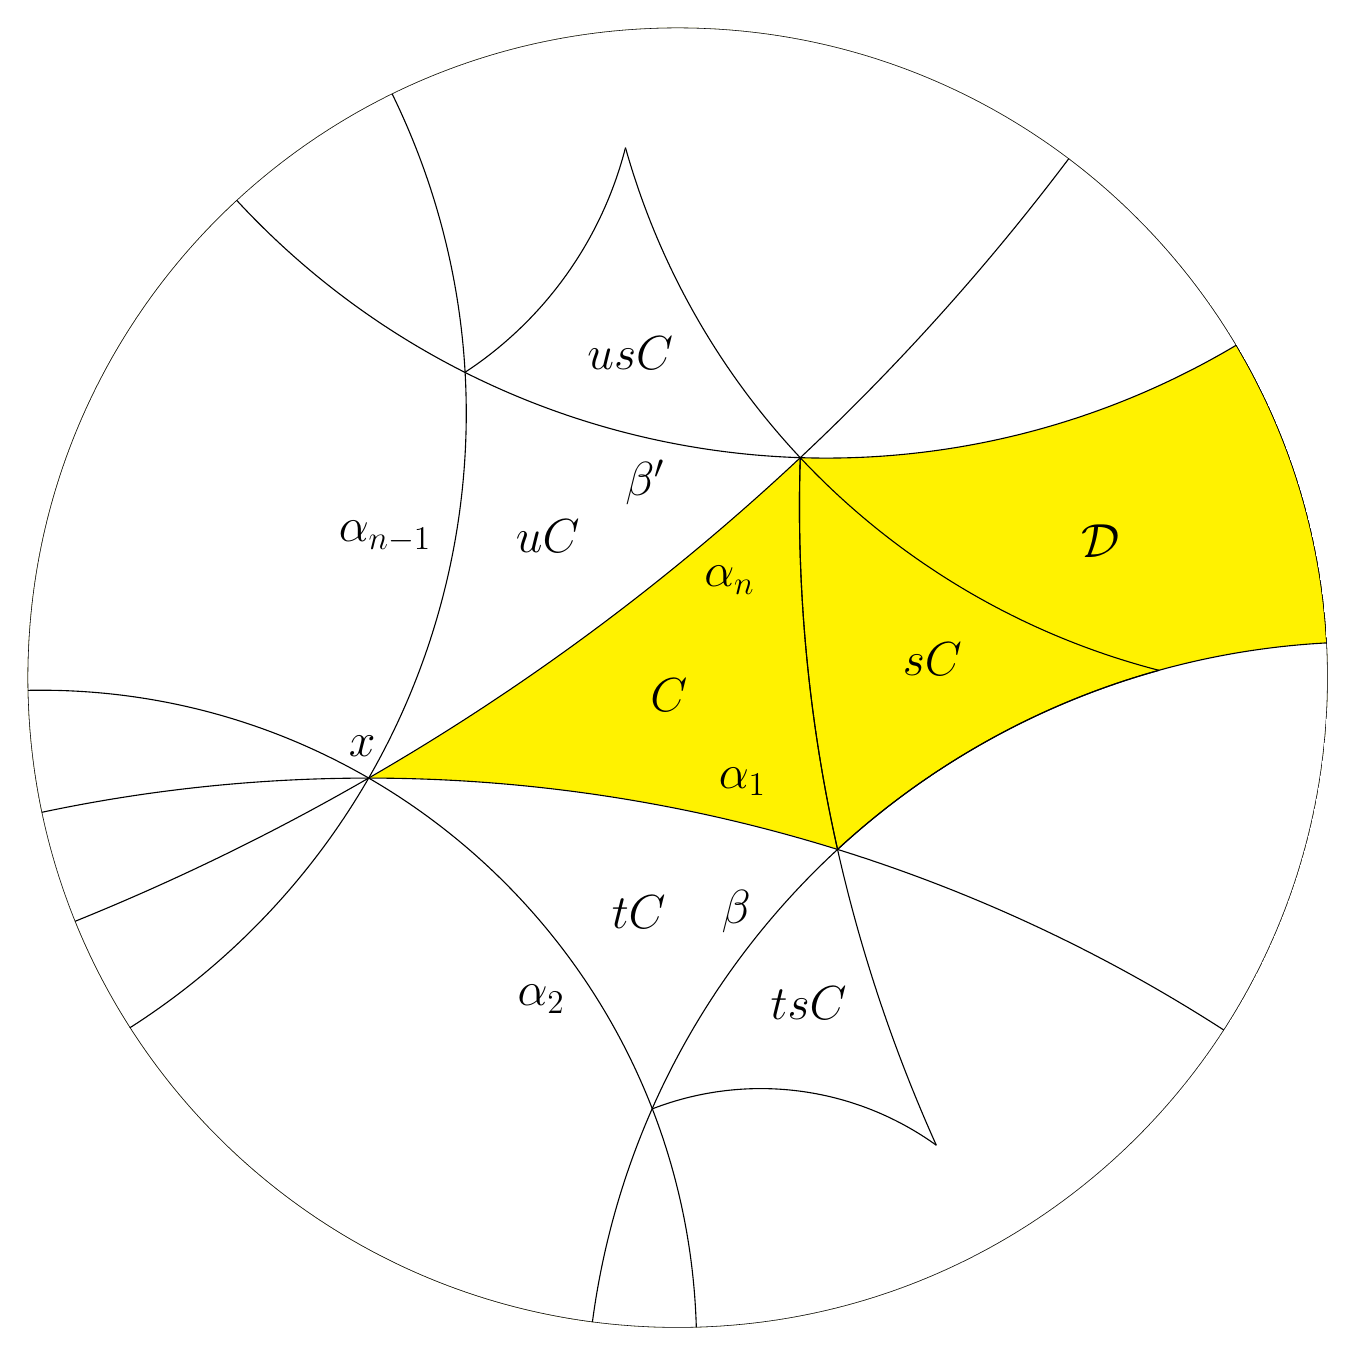
\begin{tikzpicture}[scale=8.255]

\LARGE
\clip (0,0) circle (1);

\draw[fill=yellow] (0,0) circle (1);
\fill[fill=white] (-2.2791250250110378,2.9693405967658713) circle (3.6071310565646857);
\fill[fill=white] (-0.47550398689075224,-2.5816341795598716) circle (2.427125682493754);
\fill[fill=white] (0.2280854151069161,1.5721027730090256) circle (1.234313609050456);
\fill[fill=white] (1.0630193146278248,-1.1494226757936716) circle (1.204650385340284);
\draw (0.65,0.21) node {$\mathcal{D}$};



\draw (0,0) circle (1);
%Chamber: C
\draw (-0.013657570534325638,-0.026767476865492412) node {$C$};

%Vertices:
% type s: (-0.47552825814757677,-0.1545084971874737)
% type u: (0.24595767065764057,-0.26421489179421187)
% type t: (0.18859787588695928,0.33842095838520836)
\draw (0.08,0.15) node {\LARGE $\alpha_n$};
\draw (0.1,-0.16) node {\LARGE $\alpha_1$};
\draw (-0.48552825814757677,-0.1445084971874737) node[above] {\LARGE $x$};

%Walls
% s wall:
%\draw(0.2905630711827432,0.9568558416317748) arc (163.10833072538367:208.48856328086245:2.39173576389932);
% s panel:
\draw(0.18859787588695928,0.33842095838520836) arc (178.16670947737816:192.70752950580447:2.39173576389932);
%Drawing Center: (2.5791094085094426,0.26190575261558335)
%Drawing Radius: (2.39173576389932)
% u wall:
\draw(-0.9270972812105227,-0.3748207987452894) arc (-67.98676245901322:-36.99696875053164:3.6071310565646852);
% u panel:
%\draw(-0.47552825814757677,-0.1545084971874737) arc (-59.999427042204886:-46.833290522621894:3.6071310565646857);
%Drawing Center: (-2.2791250250110378,2.9693405967658713)
%Drawing Radius: (3.6071310565646857)

% t wall:
\draw(0.8402986250578879,-0.5421238057176822) arc (57.17166713485727:101.95596676115449:2.427125682493754);
% t panel:
%\draw(-0.47552825814757677,-0.1545084971874737) arc (90.00057295779513:72.70752950580444:2.427125682493754);
%Drawing Center: (-0.47550398689075224,-2.5816341795598716)
%Drawing Radius: (2.427125682493754)

%%%%%%%%%%%%%%%%%%%%
%Chamber: uC
\draw (-0.2,0.2178845617204473) node {$uC$};
\draw (-0.45,0.217) node {$\alpha_{n-1}$};

%Vertices:
% type u: (-0.32718848187847954,0.46974122396360724)
% type s: (-0.47552825814757677,-0.1545084971874737)
% type t: (0.18859787588695928,0.33842095838520836)
\draw (-0.05,0.3) node {\LARGE $\beta'$};

%Walls
% u wall:
%\draw(-0.9270972812105227,-0.3748207987452894) arc (-67.98676245901322:-36.99696875053164:3.6071310565646852);
% u panel:
%\draw(-0.47552825814757677,-0.1545084971874737) arc (-59.999427042204886:-46.833290522621894:3.6071310565646857);
%Drawing Center: (-2.2791250250110378,2.9693405967658713)
%Drawing Radius: (3.6071310565646857)
% s wall:
\draw(-0.6785662839099904,0.7345391741361287) arc (-137.26829125436254:-59.241800373848996:1.234313609050456);
% s panel:
%\draw(0.18859787588695928,0.33842095838520836) arc (-91.83329052262194:-116.73499190878844:1.234313609050456);
%Drawing Center: (0.2280854151069161,1.5721027730090256)
%Drawing Radius: (1.234313609050456)

% t wall:
\draw(-0.8426075317169581,-0.5385281306430105) arc (-57.41650157433108:26.061166174123002:1.1208449642100555);
% t panel:
%\draw(-0.47552825814757677,-0.1545084971874737) arc (-29.999427042204896:3.2650080912115933:1.1208449642100555);
%Drawing Center: (-1.4462140750336314,0.4059042780874064)
%Drawing Radius: (1.1208449642100555)

%%%%%%%%%%%%%%%%%%%%
%Chamber: sC
\draw (0.3917126995200134,0.02849340030488451) node {$sC$};

%Vertices:
% type s: (0.7405825520154404,0.011274134323657025)
% type u: (0.24595767065764057,-0.26421489179421187)
% type t: (0.18859787588695928,0.33842095838520836)

%Walls
% s wall:
%\draw(0.2905630711827432,0.9568558416317748) arc (163.10833072538367:208.48856328086245:2.39173576389932);
% s panel:
\draw(0.18859787588695928,0.33842095838520836) arc (178.16670947737816:192.70752950580447:2.39173576389932);
%Drawing Center: (2.5791094085094426,0.26190575261558335)
%Drawing Radius: (2.39173576389932)
% u wall:
%\draw(-0.11532333779152709,0.9933280061292047) arc (-173.37772497766048:-91.42776573090109:1.1513834950667081);
% u panel:
\draw(0.7405825520154404,0.011274134323657025) arc (-104.47492746008183:-136.8332905226218:1.1513834950667081);
%Drawing Center: (1.0283781336531612,1.1261093938583715)
%Drawing Radius: (1.1513834950667081)
% t wall:
%\draw(0.9985677252158665,0.053502319175994184) arc (93.06692144755692:172.46016269931752:1.204650385340284);
% t panel:
\draw(0.7405825520154404,0.011274134323657025) arc (105.52507253991814:132.70752950580453:1.204650385340284);
%Drawing Center: (1.0630193146278266,-1.1494226757936699)
%Drawing Radius: (1.204650385340284)

%%%%%%%%%%%%%%%%%%%%
%Chamber: tC
\draw (-0.06,-0.360722068063557) node {$tC$};
\draw (-0.15,-0.45) node[below left] {$\alpha_2$};

%Vertices:
% type t: (-0.03925384843411938,-0.6634428152089855)
% type s: (-0.47552825814757677,-0.1545084971874737)
% type u: (0.24595767065764057,-0.26421489179421187)
\draw (0.09,-0.36) node {\LARGE $\beta$};

%Walls
% t wall:
%\draw(0.8402986250578879,-0.5421238057176822) arc (57.17166713485727:101.95596676115449:2.427125682493754);
% t panel:
%\draw(-0.47552825814757677,-0.1545084971874737) arc (90.00057295779513:72.70752950580444:2.427125682493754);
%Drawing Center: (-0.47550398689075224,-2.5816341795598716)
%Drawing Radius: (2.427125682493754)
% s wall:
\draw(0.9985677252158665,0.053502319175992685) arc (93.06692144755682:172.46016269931746:1.204650385340284);
% s panel:
%\draw(-0.03925384843411938,-0.6634428152089855) arc (156.207856243496:132.70752950580442:1.204650385340284);
%Drawing Center: (1.0630193146278248,-1.1494226757936716)
%Drawing Radius: (1.204650385340284)

% u wall:
\draw(0.028682084827241383,-0.9995885843735728) arc (1.6435878136565714:91.11697453255913:1.0092336344357047);
% u panel:
%\draw(-0.47552825814757677,-0.1545084971874737) arc (60.00057295779514:21.207856243496035:1.0092336344357047);
%Drawing Center: (-0.9801363351205405,-1.0285355090869626)
%Drawing Radius: (1.0092336344357047)


%%%%%%%%%%%%%%%%%%%%

%Chamber: suC
\draw (-0.0729586568911132,0.5) node {$usC$};

%Vertices:
% type s: (-0.08028536468181936,0.8153857221311153)
% type u: (-0.32718848187847954,0.46974122396360724)
% type t: (0.18859787588695928,0.33842095838520836)

%Walls
% s wall:
%\draw(-0.6785662839099904,0.7345391741361287) arc (-137.26829125436254:-59.241800373848996:1.234313609050456);
% s panel:
%\draw(0.18859787588695928,0.33842095838520836) arc (-91.83329052262194:-116.73499190878844:1.234313609050456);
%Drawing Center: (0.2280854151069161,1.5721027730090256)
%Drawing Radius: (1.234313609050456)
% u wall:
%\draw(-0.11532333779152543,0.9933280061292049) arc (-173.3777249776606:-91.42776573090123:1.151383495066709);
% u panel:
\draw(-0.08028536468181936,0.8153857221311153) arc (-164.34347868402858:-136.83329052262198:1.151383495066709);
%Drawing Center: (1.0283781336531639,1.12610939385837)
%Drawing Radius: (1.151383495066709)
% t wall:
%\draw(-0.9024526076389858,0.4307891490806086) arc (-115.51765195249614:3.620440658860526:0.5874229483600517);
% t panel:
\draw(-0.08028536468181936,0.8153857221311153) arc (-14.343478684028579:-56.73499190878849:0.5874229483600517);
%Drawing Center: (-0.649397175564537,0.9609105206151186)
%Drawing Radius: (0.5874229483600517)

%%%%%%%%%%%%%%%%%%%%
%Chamber: stC
\draw (0.20154262506178333,-0.5) node {$tsC$};

%Vertices:
% type s: (0.39792405296182876,-0.7193334685021296)
% type t: (-0.03925384843411938,-0.6634428152089855)
% type u: (0.24595767065764057,-0.26421489179421187)

%Walls
% s wall:
%\draw(0.9985677252158665,0.053502319175992685) arc (93.06692144755682:172.46016269931746:1.204650385340284);
% s panel:
%\draw(-0.03925384843411938,-0.6634428152089855) arc (156.207856243496:132.70752950580442:1.204650385340284);
%Drawing Center: (1.0630193146278248,-1.1494226757936716)
%Drawing Radius: (1.204650385340284)
% t wall:
%\draw(0.29056307118274743,0.9568558416317736) arc (163.10833072538344:208.48856328086237:2.39173576389931);
% t panel:
\draw(0.39792405296182876,-0.7193334685021296) arc (-155.7786814577639:-167.29247049419564:2.39173576389931);
%Drawing Center: (2.5791094085094346,0.26190575261557547)
%Drawing Radius: (2.39173576389931)
% u wall:
%\draw(0.5218877984810576,-0.8530141416158321) arc (31.458966684034202:161.8713504707822:0.46193373430200985);
% u panel:
\draw(0.39792405296182876,-0.7193334685021296) arc (54.22131854223611:111.20785624349597:0.46193373430200996);
%Drawing Center: (0.12785179063203292,-1.094091721254842)
%Drawing Radius: (0.46193373430200996)

%%%%%%%%%%%%%%%%%%%%
\end{tikzpicture}
\end{document}
